% !TEX root = ../Thesis.tex
% !TEX output_directory
\documentclass[11pt,a4paper,english,greek,twoside]{../Thesis}
\begin{document}
\chapter{Υλοποίηση SSVEP διεπαφής - Hardware} \label{chap:SSVEP_implementation}
Στο κεφάλαιο 2, έγινε μια γενική περιγραφή των SSVEP σημάτων, και πως μπορούμε να τα χρησιμοποιήσουμε για την υλοποίηση διεπαφών μεταξύ εγκεφάλου και υπολογιστή. Σε αυτή την ενότητα θα γίνει παρουσίαση και αναλυτική περιγραφή της SSVEP διεπαφής που υλοποιήθηκε στα πλαίσια αυτής της διπλωματικής εργασίας.

\section{Παρόμοιες εργασίες - Ανασκόπηση Βιβλιογραφίας}

Ergasies pou kanoun xrisi EMOTIV EPOC

Η πιο cited δημοσίευση στο θέμα Epoc - SSVEP αναφέρει τρελά αποτελέσματα, χωρίς να περιγράφει καθόλου μέθοδο τακτικές λεπτομερειες κλπ.
[[
Y. Liu, X. Jiang, T. Cao, F. Wan, P.U. Mak, P.I. Mak, M.I. Vai, Implementation of SSVEP based BCI with Emotiv EPOC, in 2012 IEEE International Conference on Virtual Environments Human-Computer Interfaces and Measurement Systems (VECIMS) (IEEE, 2012), pp. 34–37
]]

Φαίνεται πως το Epoc αποδίδει καλά στα σήματα P300 αν και δεν έχει ηλεκτρόδια εκει που πρεπει Debener S, Minow F, Emkes R, Gandras K, de Vos M: How about taking a low-cost, small, and wireless EEG for a walk?. Psychophysiology. 2012, 49: 1617-1621.
[[
[HTML] Performance of the Emotiv Epoc headset for P300-based applications
M Duvinage, T

D. Matthieu, C. Thierry, P. Mathieu, A P300-based quantitative comparison between the Emotiv EPOC headset and a medical EEG device. Int. J. Biomed. Eng. 12(56), 201 (2013)
]]

ερευνα απο San Diego
[[
https://jneuroengrehab.biomedcentral.com/articles/10.1186/1743-0003-11-119
chance level (25\%) 
Edw perpataei aytos, alla leei kai ta apotelesmata tou gia otan ειναι ακίνητος
standing condition (accuracy: 76.60 ± 21.74\%, ITR: 14.38 ± 9.04).  Ta dika mas einai kalytera.
Decision time standing: 4.34 ± 0.08 s, emas einai ligotero

The amplitude of SSVEP has been found to be largely modulated by visual spatial attention [28]. As a consequence, the loss of focus could reduce visual attention and thereby lead to the decreased SSVEP amplitude.
Ara na dokimasw sto real time na mhn mou deixnei to feedback gia na mn exw distract
]]

http://sci-hub.tw/https://ieeexplore.ieee.org/abstract/document/6843587/
edw dokimasan high freq που ειναι πιο δυσκολες γενικα, kai petyxan 73.75% 11.36 ITR . xeirotera ομως ap to prohgoumeno. παλι δν περιγραφουν τπτ απο την μεθοδο τους. 

Controlling mobile Spykee robot using Emotiv neuro headset 2013 china
cited by 19
Edw οι τυπαδες πανε να εξαγουν 4 εντολες με mental controls, οχι με προκλητα δυναμικα δλδ, και στην συνεχεια αναρρωτιουνται πως αλλιως μπορουνε. προτεινουν SSVEP, αλλα καταλήγουν πως to emotiv dn anixneyei ssvep (οτι να ναι), επειδη τα Ο1 και Ο2 δεν ειναι καταλληλα για αυτη τη δουλεια (οτι να ναι παλι)

%http://www.koreascience.or.kr/article/ArticleFullRecord.jsp?cn=PJJNBT_2015_v25n3_254
εδω πετυχαινουν 70\% με LDA kai SVM





\section{Υλικό}
%%%%%%%%%%%%%%%%%%%%%%%% General
\subsection{Εγκεφαλογράφος Emotiv Epoc}
\subsubsection{Περιγραφή}
\par Το σύστημα  Epoc από την εταιρεία Emotiv Systems, δημιουργήθηκε το 2009 και είναι ένας χαμηλού κόστους φορητός ασύρματος εγκεφαλογράφος, ο οποίος προορίζεται για χρήση σε παιχνίδια (gaming EEG system) και απλές εφαρμογές και όχι για να αντικαταστήσει τους κατά πολύ ακριβότερους εγκεφαλογράφους που χρησιμοποιούνται σε ιατρικές εφαρμογές . Το EPOC είναι μια πολύ συμπαγής κατασκευή, καθώς τα ηλεκτρόδια, ο ενισχυτής, τα κυκλώματα επεξεργασίας σήματος (DSP chips) αλλά και το σύστημα επικοινωνίας Bluetooth, είναι όλα ενσωματωμένα σε μια πλακέτα μέσα στην συσκευή, καθιστώντας το πολύ εύκολο στην μεταφορά και την χρήση. 
\par Προσφέρει καταγραφή απο 16 ηλεκτρόδια τοποθετημένα σε πλαστικούς βραχίονες, και  καλύπτουν μια σχετικά ευρεία περιοχή του εγκεφάλου. Πιο συγκεκριμένα οι θέσεις που καλύπτουν τα ηλεκτρόδια, σύμφωνα με το διεθνές σύστημα 10-20 είναι οι : AF3, F7, F3, FC5, T7, P7, O1, O2, P8, T8, FC6, F4, F8, FC4, P3, και P4. Ο αισθητήρας στην θέση P3 (CMS) χρησιμοποιείται ώς ηλεκτρόδιο αναφοράς (reference), ενώ ο P4 (DRL) δρα ως feed-forward αντισταθμιστής των εξωτερικών αλλαγών που επηρεάζουν το συνολικό δυναμικό του σώματος, όπως οι παρεμβολές των 50Hz της τροφοδοσίας, οι μετασχηματιστές κ.α. 
%Eikona 10-20 me tous aisthitires και το ΕΜΟΤΙΒ
 \begin{figure}[H]
    \centering     %%% not \center
    \subfigure[]{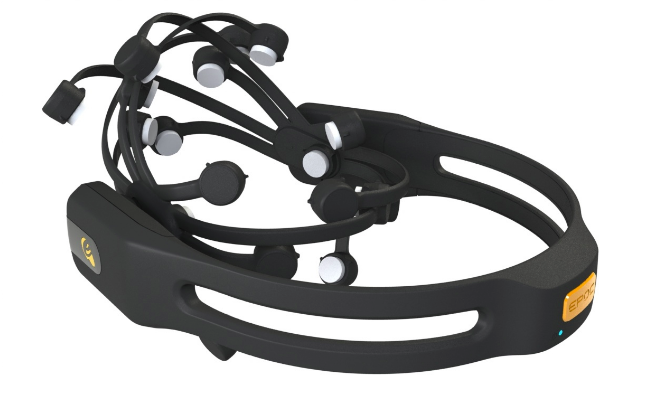
\includegraphics[scale = 0.35]{{{ImagesSSVEP/emotiv}.png}}}
    \subfigure[]{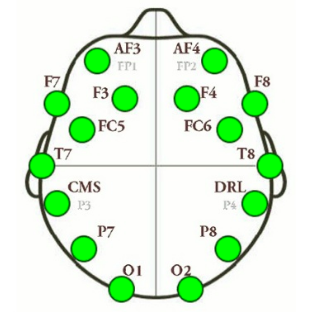
\includegraphics[width=60mm]{{{ImagesSSVEP/emotiv_elec_pos}.png}}}
    \caption{Ο ασύρματος εγκεφαλογράφος Epoc της εταιρείας Emotiv (a), και οι θέσεις που καλύπτουν τα 16 ηλεκτρόδια του, σύμφωνα με το σύστημα 10-20 (b).}
    \end{figure}
\par Επιπλέον, ενσωματωμένα μέσα στον εγκεφαλογράφο βρίσκονται τόσο αναλογικά όσο και ψηφιακά φίλτρα. Αρχικά το σήμα κάθε αισθητήρα φιλτράρεται από ένα υψηπερατό C-R φίλτρο με συχνότητα αποκοπής στα 0.16Hz, έπειτα περνάει απο ένα στάδιο προ-ενίσχυσης και στην συνέχεια απο ένα βαθυπερατό φίλτρο με συχνότητα αποκοπής 83Hz. Στο επόμενο στάδιο γίνεται δειγματοληψία του σήματος από έναν αναλογικό σε ψηφιακό μετατροπέα (ADC) με συχνότητα δειγματοληψίας 2048Hz και το σήμα φιλτράρεται από ένα ψηφιακό sinc φίλτρο 5ης τάξης για την αφαίρεση της συνιστώσας των 50Hz της τροφοδοσίας, και τέλος γίνεται υποδειγματοληψία στα 128Hz. Αν και αυτή η δειγματοληψία (128Hz) είναι ικανή για την καταγραφή συχνοτήτων ως και $64Hz$, εύρος που περιλαμβάνει την πλειοψηφία εγκεφαλικής λειτουργίας, παραμένει σημαντικά μικρότερος από τον αντίστοιχο ρυθμό δειγματοληψίας άλλων εγκεφαλογράφων αγγίζουν μέχρι και τα 2048Hz.

\subsubsection{Ηλεκτρόδια}
\par Τα ηλεκτρόδια με τα οποία είναι εξοπλισμένος ο EPOC, είναι ‘υγρού’ τύπου, παρόλαυτα διαφέρουν αρκετά ως προς την δομή συγκριτικά με τα ευρέως χρησιμοποιούμενα Ag/Ag-Cl που αναφέρθηκαν στην παράγραφο 1.2
Τα συγκεκριμένα, αποτελούνται από ένα κυκλικό κομμάτι από ανοξείδωτο ατσάλι, επικαλυμμένο από μια λεπτή στρώση χρυσού. Η τελευταία στρώση αποτελείται από ένα πολυμερές υλικό υποδοχέα (polymer host) σε συνδυασμό με ένα ηλεκτρολυτικό, μη πολικό υλικό για το οποίο η εταιρεία δεν δίνει παραπάνω πληροφορίες. Η επαφή με το δέρμα γίνεται μέσω μιας κυλινδρικής τσόχας πολυεστέρα (felt pad), την οποία σε κάθε χρήση, διαποτίζουμε σε αλατούχο διάλυμα (saline) για την ελάττωσή της αντίστασης επαφής.
\par Το βασικό πρόβλημα από το οποίο υποφέρουν τα ηλεκτρόδια αυτά είναι η οξείδωση.  Παρά την λεπτή στρώση χρυσού που θα έπρεπε να την αποτρέπει, φαίνεται πως ένα απο τα άλλα υλικά της επίστρωσης, αντιδρά με το αλατούχο διάλυμα και την προκαλεί. Σύμφωνα με το τεχνικό επιτελείο της εταιρείας, δεν έχει γίνει χημική ανάλυση για να διαπιστωθεί ακριβώς η αιτία της. Τέλος, επειδή παρατηρήθηκε πως η οξείδωση ξεκινάει πάντα από την περιφέρεια του ηλεκτροδίου, είναι πολύ πιθανόν να μη είναι επαρκής η χρυσή επίστρωση σε αυτό το σημείο και να εκτίθεται το ανοξείδωτο ατσάλι στο αλατούχο διάλυμα, το οποίο αν είναι χαμηλής ποιότητας μπορεί να προκαλέσει την οξείδωση.
\par Η σημαντική επίπτωση που έχει η οξείδωση των ηλεκτροδίων δεν αφορά τόσο την ποιότητα του σήματος, καθώς δεν επηρεάζεται η αγωγιμότητα του ηλεκτροδίου, όσο την μηχανική δομή και αντοχή του. Παρατηρήθηκε πως μετά από το χρονικό διάστημα λίγων μηνών ξεκίνησε η φθορά στο πλαστικό σπείρωμα του πλαστικού στηρίγματος του ηλεκτροδίου, ενώ σε παλιότερα ηλεκτρόδια που υπήρχαν στο εργαστήριο, το πλαστικό στήριγμα είχε σπάσει καθιστώντας το ηλεκτρόδιο εντελώς άχρηστο.
\begin{figure}[H]
    \centering     %%% not \center
    \subfigure[]{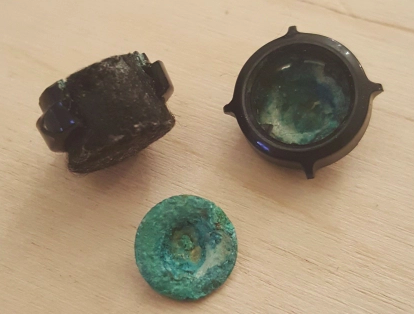
\includegraphics[width=60mm]{{{ImagesSSVEP/sapia_elec}.png}}}
    \subfigure[]{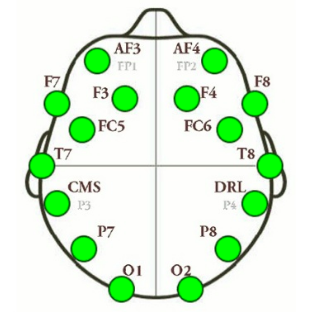
\includegraphics[width=60mm]{{{ImagesSSVEP/emotiv_elec_pos}.png}}}
    \caption{Ο ασύρματος εγκεφαλογράφος Epoc της εταιρείας Emotiv (a), και οι θέσεις που καλύπτουν τα 16 ηλεκτρόδια του, σύμφωνα με το σύστημα 10-20 (b).}
    \end{figure}
\par \textcolor{red}{(Να βάλω συμβουλες για χρηση και διατηρηση ηλεκτροδίων ? )}

\subsubsection{Λογισμικό}
\textbf{Emotiv Sofware}
\par Μαζί με τον εγκεφαλογράφο Epoc, η Emotiv παρέχει μια σουίτα λογισμικού που προσφέρει στον χρήστη μια πληθώρα υπηρεσιών, άλλες δωρεάν και άλλες επί πληρωμή. 
Η βασική και δωρεάν εφαρμογή, είναι η EMOTIV Xavier Control Panel, η οποία βοηθάει τον χρήστη να κάνει την εγκατάσταση του Epoc, και να μάθει να το χρησιμοποιεί Δίνεται η δυνατότητα στον χρήστη να παρακολουθεί την ποιότητα επαφής των ηλεκτροδίων με το δέρμα αναπαριστώντας με πράσινο χρώμα την καλή ποιότητα, τις ενδιάμεσες καταστάσεις με κίτρινο και κόκκινο, ενώ μαύρο χρησιμοποιείται όταν πρακτικά λαμβάνεται μόνο θόρυβος.

\par Μια άλλη λειτουργία που παρέχεται, είναι ο υπολογισμός πέντε μετρικών εγκεφαλικής λειτουργίας σε πραγματικό χρόνο σχετικά με την συμμετοχή, την συγκέντρωση, το ενδιαφέρον, τη χαλάρωση, και το άγχος, που βιώνει ο χρήστης..

\par Τέλος παρέχεται ένα σύστημα το οποίο είναι ικανό να εκπαιδευθεί από τον κάθε χρήστη ξεχωριστά, έτσι ώστε να ξεχωρίζει συγκεκριμένες σκέψεις και να τις αντιστοιχίζει σε ξεχωριστές λειτουργίες που θα επιλέξει ο χρήστης, όπως η μετακίνηση και περιστροφή ενός εικονικού αντικειμένου ή ο έλεγχος του δείκτη του ποντικιού. Η επιτυχία αυτού του συστήματος εξαρτάται σε μεγάλο βαθμό από τον χρόνο που θα επενδύσει κάποιος στην εκπαίδευση του, καθώς και από την ικανότητα του να συγκεντρώνεται και να διαχωρίζει τις σκέψεις του. Ενδεικτικά μετά από ένα χρονικό διάστημα 10 λεπτών, επιτεύχθηκε η μετακίνηση ενός εικονικού τρισδιάστατου κύβου μπροστά και πίσω κατά βούληση, ωστόσο όταν συμπεριλήφθηκαν παραπάνω εντολές (περιστροφή δεξιόστροφη και αριστερόστροφη), τότε ήταν σχεδόν αδύνατη η μετακίνηση κύβου.
\begin{figure}[H]
    \centering     %%% not \center
    \subfigure[]{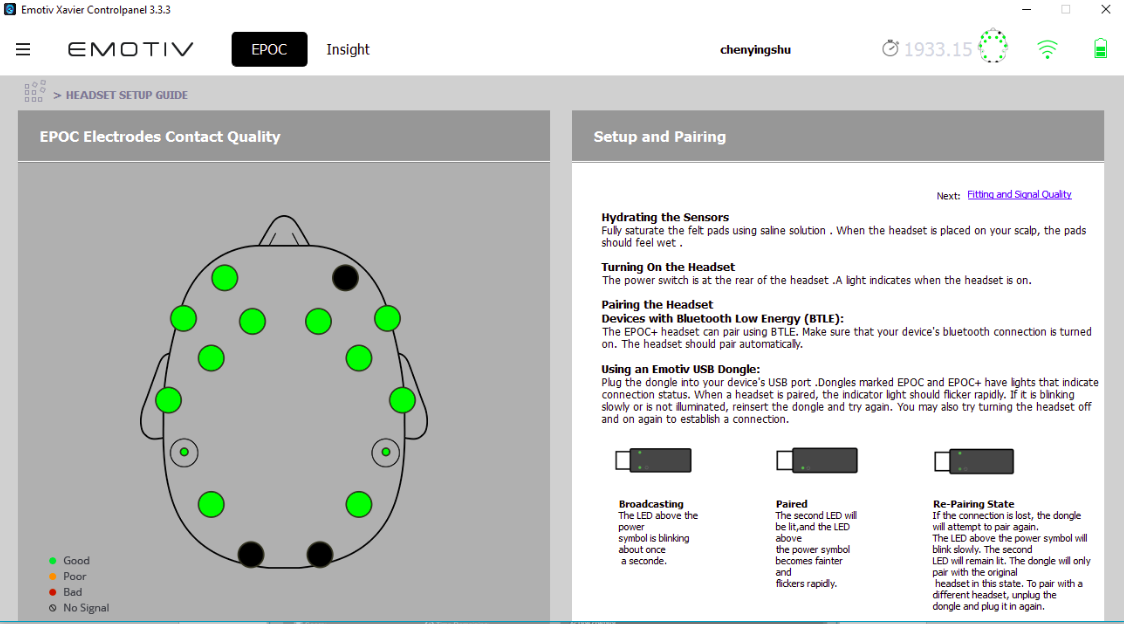
\includegraphics[width=90mm]{{{ImagesSSVEP/xavier_quality}.png}}}
    \subfigure[]{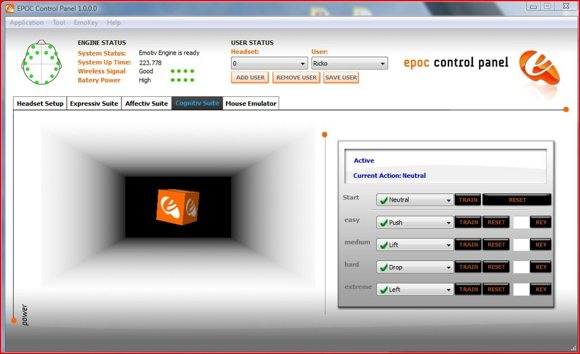
\includegraphics[width=90mm]{{{ImagesSSVEP/xavier_cube}.jpg}}}
    \caption{Το λογισμικό ελέγχου που συνοδεύει το Epoc, παρέχει ενδείξεις για την ποιότητα επαφής κάθε ηλεκτροδίου, την στάθμη της μπαταρίας καθώς και την ποιότητα της bluetooth σύνδεσης (a). Ο εικονικός κύβος που ο χρήστης μαθαίνει να ελέγχει με την σκέψη του (b). }
    \end{figure}

\textbf{Emokit}
\par Προκειμένου όμως ένας χρήστης να αποκτήσει πρόσβαση στις μετρήσεις κάθε αισθητήρα ξεχωριστά, δηλαδή στο εγκεφαλογράφημα αυτό καθ’ αυτό, θα πρέπει αγοράσει την ερευνητική έκδοση του EPOC (research Edition). Με αυτή την έκδοση, η Emotiv παρέχει το ερευνητικό κιτ ανάπτυξης λογισμικού (research SDK) το οποίο μπορεί να χρησιμοποιηθεί με μια πληθώρα προγραμματιστικών γλωσσών (C++, Python, Matlab, Java, C\#) για την επεξεργασία των εγκεφαλικών σημάτων. Το γεγονός όμως πως ο εγκεφαλογράφος που υπήρχε στο εργαστήριο δεν ήταν η ερευνητική έκδοση, μας οδήγησε στην εύρεση λύσης σε ελεύθερο λογισμικό το οποίο να παρέχει δυνατότητες παρόμοιες με αυτές του research SDK απο την Emotiv. Μια τέτοια βιβλιοθήκη είναι η Emokit και δημιουργήθηκε από την ομάδα προγραμματιστών στην OpenYou, και δίνει πρόσβαση στις μετρήσεις των αισθητήρων, την ποιότητα της επαφής και την στάθμη της μπαταρίας της συσκευής. Επιπλέον, δίνεται η δυνατότητα εξαγωγής των αποτελεσμάτων σε μορφή csv, καθώς και η αντίστροφη διαδικασία, κατά την οποία ένα csv αρχείο “διαβάζεται” σε πραγματικό χρόνο, προσομοιώνοντας τον πραγματικό εγκεφαλογράφο.

\par Στην βιβλιοθήκη συμπεριλαμβάνονται και κάποια script που υποδεικνύουν τους βασικούς τρόπους χρήσης. Αρχικά τρέχοντας το example.py εμφανίζεται ένας πίνακας με την τιμή, και την ποιότητα για κάθε ηλεκτρόδιο, τις τιμές για τον γυροσκοπικό αισθητήρα καθώς και την στάθμη της μπαταρίας.

\par Αυτού του είδους η απεικόνιση είναι μάλλον άβολη για μελέτη των εγκεφαλικών σημάτων και πιο πολύ χρησιμεύει ως ένας γρήγορος έλεγχος της ποιότητας σύνδεσης του EPOC με τον υπολογιστή.
Ένας πολύ διαφορετικό τρόπος απεικόνισης υλοποιείται στο αρχείο render.py όπου κάνοντας χρήση της βιβλιοθήκης pygame απεικονίζονται σε πραγματικό χρόνο τα διαγράμματα τιμών για κάθε ηλεκτρόδιο ξεχωριστά. Επίσης το χρώμα της γραφικής παράστασης εξαρτάται από την ποιότητα της επαφής του ηλεκτροδίου με το δέρμα. 
\begin{figure}[H]
    \centering     %%% not \center
    \subfigure[]{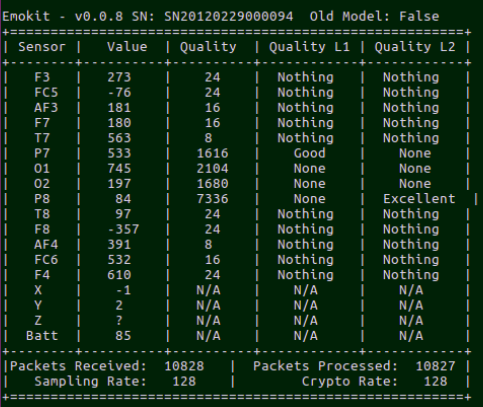
\includegraphics[width=70mm]{{{ImagesSSVEP/examplepy}.png}}}
    \subfigure[]{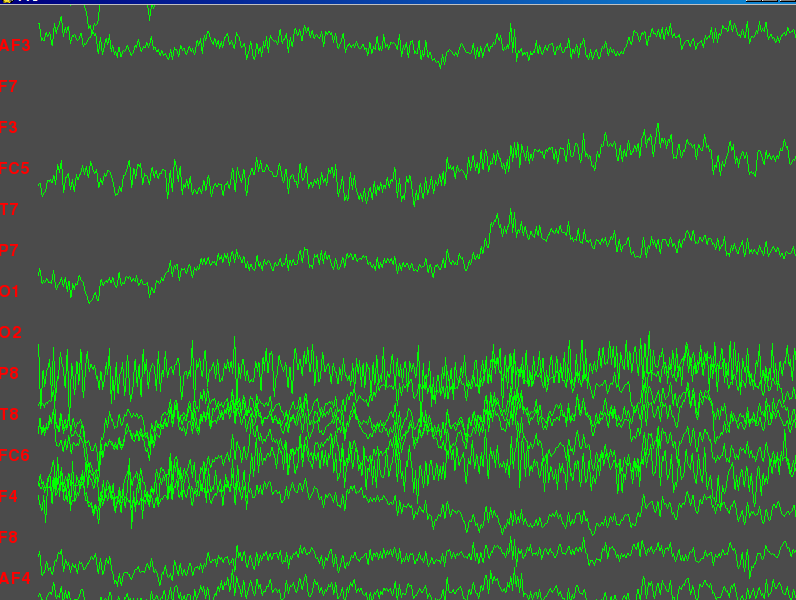
\includegraphics[width=70mm]{{{ImagesSSVEP/render}.png}}}
    \caption{Ο πίνακας τιμών και ποιότητας για κάθε αισθητήρα (a) και η γραφική διεπαφή οπτικοποίησης των εγκεφαλικών σημάτων (b) που παρέχονται από την βιβλιοθήκη Emokit.}
    \label{fig:render}
\end{figure}
\par Παρότι αυτού του είδους η απεικόνιση είναι πολύ χρήσιμη, ένα βασικό πρόβλημα που φαίνεται και στην εικόνα \ref{fig:render}, είναι πως τα σήματα που δίνει το EPOC περιέχουν offset, με αποτέλεσμα πολλές φορές οι γραφικές παραστάσεις να μετατοπίζονται στον κάθετο άξονα και να μπερδεύονται μεταξύ τους. Επίσης δεν παρέχεται καθόλου συχνοτική πληροφορία για κάθε κανάλι, πράγμα το οποίο θα βοηθούσε στην γρήγορη οπτικοποίηση των SSVEP σημάτων.
\par Κρίθηκε σημαντικό λοιπόν, στα πλαίσια της παρούσας διπλωματικής εργασίας, να αναπτυχθεί μια γραφική διεπαφή για την οπτικοποίηση των εγκεφαλικών σημάτων, σε Python 2.7,  με τα εξής χαρακτηριστικά :
\begin{itemize}
    \item{Χρήση του εργαλείου pyqtgraph για την δημιουργία του γραφικού περιβάλλοντος}
    \item{Ενσωμάτωση φίλτρων για την αφαίρεση του offset, και λοιπών συχνοτήτων που μπορεί να μην ενδιαφέρουν.}
    \item{Εμφάνιση του διαγράμματος Power Spectrum Density για κάθε κανάλι,  με δυνατότητα επιλογής του παραθύρου υπολογισμού του μετασχηματισμού Fourier}
    \item{Τα χρώματα των γραφικών παραστάσεων να βασίζονται στην τιμή ποιότητας για κάθε κανάλι.}
    \item{Ενδείξεις για την ακριβή τιμή της ποιότητας καθώς και για το συχνοτικό peak, στο γράφημα του χρόνου και της συχνότητας αντίστοιχα.}
\end{itemize}

\begin{figure}[H]
    \centering     %%% not \center
    \subfigure[]{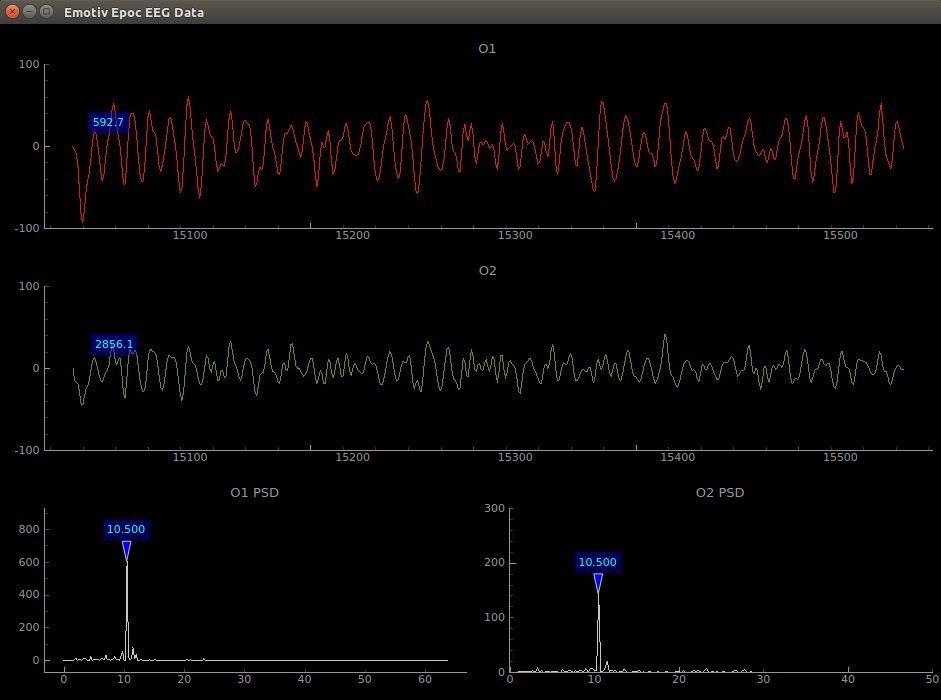
\includegraphics[width=72mm,height=50mm]{{{ImagesSSVEP/alpha_waves}.png}}}
    \subfigure[]{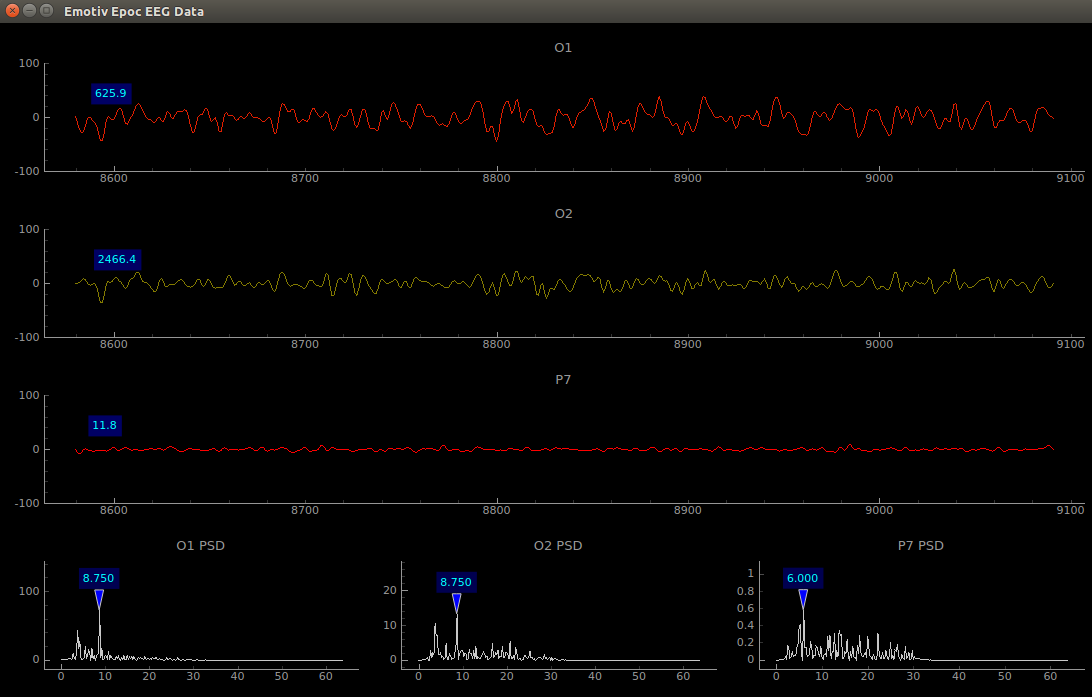
\includegraphics[width=72mm,height=50mm]{{{ImagesSSVEP/randomP7}.png}}}
    \caption{Η γραφική διεπαφή που υλοποιήσαμε για την οπτικοποίηση επιλεγμένων καναλιών στο πεδίο του χρόνου και της συχνότητας. Στην αριστερή εικόνα o χρήστης είχε κλειστά μάτια και επιλέχθηκαν τα κανάλια Ο1 και Ο2 οπού φαίνονται ξεκάθαρα τα άλφα κύματα στα $10.5Hz$, ενώ στην δεξιά εικόνα ο χρήστης άνοιξε τα μάτια του, και  προστέθηκε και το κανάλι P7.}
    \label{fig:render}
\end{figure}

\subsection{Υπολογιστής}
\par Η όλη εφαρμογή υλοποιήθηκε σε έναν φορητό υπολογιστή ASUS με επεξεργαστή Intel Pentium i7 και χρησιμοποιώντας το λειτουργικό σύστημα Ubuntu. Παρότι η βιβλιοθήκη Emokit υποστηρίζεται τόσο για Windows όσο και για Unix λειτουργικά, διάφορα προβλήματα που παρουσιάστηκαν στην επικοινωνία του EPOC με τον υπολογιστή στο Windows περιβάλλον, ώθησαν στην επιλογή του Ubuntu.

\subsection{Συστοιχίες LED}
\par Στην υποενότητα \ref{subsec:visual_stimulus} αναλύθηκαν οι πιο συχνοί τρόποι που χρησιμοποιούνται για την επίτευξη της επαναλαμβανόμενης οπτικής διέγερσης (ΕΟΔ), καθώς και τα χαρακτηριστικά της καθεμιάς. Σστην παρούσα εργασία επιλέχθηκε η μέθοδος των LEDs, καθώς οι διεπαφές που τα χρησιμοποιούν ως ΕΟΔ, επιτυγχάνουν κατά μέσο όρο υψηλότερες επιδόσεις accuracy, και ITR \cite{zhu2010survey}. Σε αυτήν την υπόενότητα θα γίνει μια παρουσίαση των LED συστοιχιών που κατασκευάστηκαν καθώς και της βάσης τους η οποία προσαρμόζεται στην οθόνη ενός φορητού υπολογιστή.

\subsubsection{Επιλογή χρώματος LED}
\par Ένας από τα βασικά χαρακτηριστικά των LED, που παίζει σημαντικό ρόλο στην ποιότητα των SSVEP σημάτων που θα προκληθούν στον εγκέφαλο, είναι το χρώμα των LED. 
ΧΧΧ
ΠΕΣ ΓΙΑ ΈΡΕΥΝΕΣ, ΓΙΑ 3 ΚΑΜΠΎΛΕΣ ΣΤΟ ΜΆΤΙ (RGB), 
Παρότι τα άσπρου χρώματος LED φαίνεται να αποδίδουν καλύτερα, σε δοκιμές που κάναμε χρησιμοποιώντας μια συστοιχία 25 LEDs, διατεταγμένα 5x5,  παρατηρήθηκε πολύ έντονη κόπωση των ματιών σε όλα τα άτομα που δοκίμασαν να κοιτάξουν τα LED. Συγκεκριμένα, ήταν αδύνατο να κρατήσουν οπτική επαφή για πάνω από 1 λεπτό, συνεπώς ενώ τα άσπρα LED παρήγαγαν πολύ δυνατά SSVEP σήματα σε όλα τα άτομα, έπρεπε να επιλεχθούν LED διαφορετικού χρώματος.
ΕΙΚΟΝΑ ΑΠΟ SSVEP WHITE LEDS
Έπειτα από δοκιμές με κόκκινα και πράσινα LED, παρατηρήθηκε πολύ μικρή διαφορά στα παραγόμενα SSVEP σήματα, συνεπώς καταλήξαμε στα πράσινα όντας τα πιο ξεκούραστα για το μάτι, ακόμα και σε πολύ δυνατές φωτεινές εντάσεις.

\par Τα LED που επιλέχθηκαν έπρεπε να ικανοποιούν δύο βασικές προυποθέσεις: 
\begin{itemize}
    \item{Nα έχουν πολύ καλή απόδοση.}
    \item{Nα έχουν ευρεία γωνία θέασης.}
\end{itemize} 
\par Τα LED που επιλέχθηκαν είναι  τα ΤΑΔΕ με γωνια θεασης ΤΑΔΕ και 

\subsubsection{Σχηματικό και Κατασκευή}
\par Στην συγκεκριμένη διεπαφή θα χρησιμοποιήσουμε 4 πηγές φωτός οπού η κάθε μία θα αναβοσβήνει με διαφορετική συχνότητα, συνεπώς θα χρειαστούν 4 συστοιχίες LED. Ο αριθμός των LED για κάθε συστοιχία επιλέχθηκε να είναι 20, σε διάταξη 5x4. Επιλέχθηκε μεγάλος αριθμός έτσι ώστε επηρεάζοντας την τροφοδοσία των led, να υπάρχει δυνατότητα πειραματισμού με την ένταση του φωτισμού, η οποία μπορεί να κυμαίνεται από αμυδρό φωτισμό των led, μέχρι πολύ δυνατή ένταση που κουράζει γρήγορα τα μάτια. Επιπλέον, σε κάθε συστοιχία προστέθηκε ένα επιπρόσθετο κόκκινο LED διαμέτρου 3mm, του οποίου η χρησιμότητα είναι διττή. Κατά την διάρκεια της offline ανάλυσης των σημάτων θα σηματοδοτεί ποια συστοιχία θα πρέπει να κοιτάξει ο χρήστης, ενώ κατά την διάρκεια της online χρήσης της διεπαφής, θα έχει τον ρόλο του feedback επισημαίνοντας την συστοιχία στην οποία ανιχνεύεται ότι έχει στραμμένο το βλέμμα του. Κάθε συστοιχία υλοποιήθηκε πάνω σε ένα stripboard όπου καθένα από αυτά θα ενσωματώνεται σε μια ξύλινη βάση που μπορεί να προσαρμόζεται σε κάθε είδους λεπτή οθόνη.

\begin{figure}[H]
    \centering     %%% not \center
    \subfigure[]{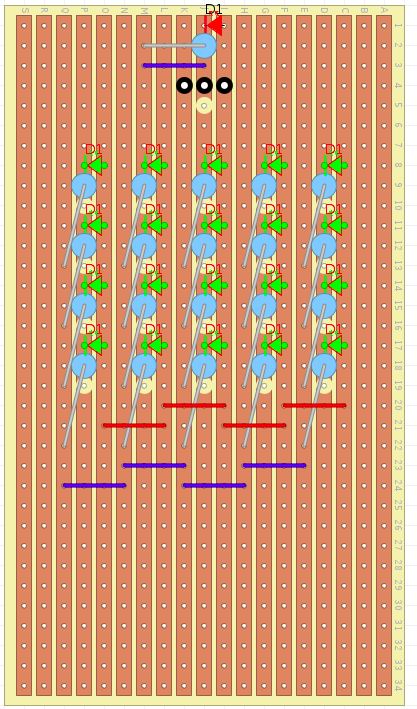
\includegraphics[width=40mm,height=60mm]{{{ImagesSSVEP/led_vero}.png}}}
    \subfigure[]{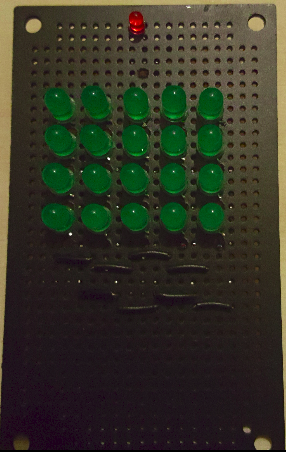
\includegraphics[width=40mm,height=60mm]{{{ImagesSSVEP/led_front2}.png}}}
    \subfigure[]{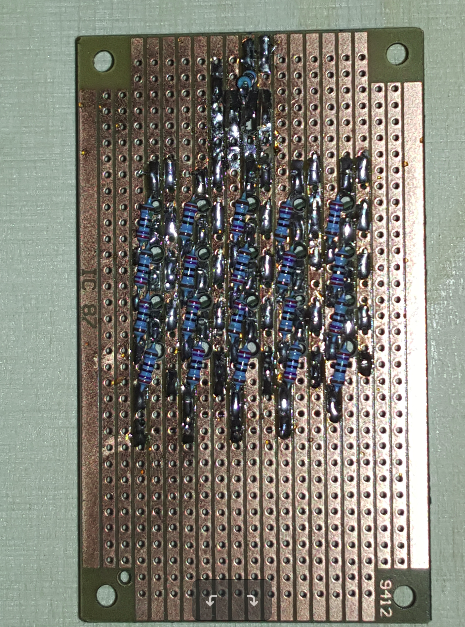
\includegraphics[width=40mm,height=60mm]{{{ImagesSSVEP/led_back}.png}}}
    \caption{Η μια από τις τέσσερις LED συστοιχίες που υλοποιήσαμε, ο φυσικός σχεδιασμός της σε stripboard (a), καθώς και η μπροστινή (b) και οπίσθια (c) όψη της τελειωμένης κατασκευής}
    \label{fig:render}
\end{figure}


\subsubsection{Κύκλωμα Οδήγησης}
\par Για τις απαιτήσεις του πειράματος απαιτούνταν ο πλήρης έλεγχος των LED, δηλαδή η δυνατότητα ξεχωριστών σημάτων ελέγχου για κάθε μια από τις 4 συστοιχίες, καθώς και για τα 4 κόκκινα LEDs συνεπώς χρειάζεται ένας μικρο-ελεγκτής με τουλάχιστον 8 ψηφιακές εξόδους, καθώς και να είναι πολύ μικρός σε μέγεθος έτσι ώστε να ενσωματωθεί εύκολα στην συνολική πλακέτα οδήγησης. Τελικώς, χρησιμοποιήθηκε ο μικροελεγκτής Arduino Nano, που παρέχει 22 ψηφιακές θύρες εισόδου/εξόδου καθώς και ειδικούς ακροδέκτες που καθιστούν εύκολη την εφαρμογή του σε πλακέτες.  
\par Κάθε συστοιχία αποτελείται από 20 LEDs και κάθε LED χρειάζεται περίπου 3mA για να παράγει επαρκή φωτεινότητα για τις απαιτήσεις του πειράματος, συνεπώς το ρεύμα που απαιτείται για την οδήγηση κάθε συστοιχίας είναι περίπου 60mA, το οποίο ξεπερνάει το μέγιστο ρέυμα που μπορει να διαχειριστεί κάθε εξοδος του Arduino (40mA). Συνεπώς θα χρησιμοποιήθούν 8 τρανζίστορ, ένα για κάθε συστοιχία και ένα για κάθε κόκκινο LED. Το κύκλωμα μπορεί να τροφοδότηθεί είτε από την θύρα Vin του arduino, που ταυτίζεται  με την  έξοδο των 5volt της θύρας USB στην οποία συνδέεται, είτε από εξωτερική DC τροφοδοσία, καθώς στο κύκλωμα περιλαμβανεται o σταθεροποιητής τάσης LM317.

\begin{figure}[H]
    \centering     %%% not \center
    \subfigure[]{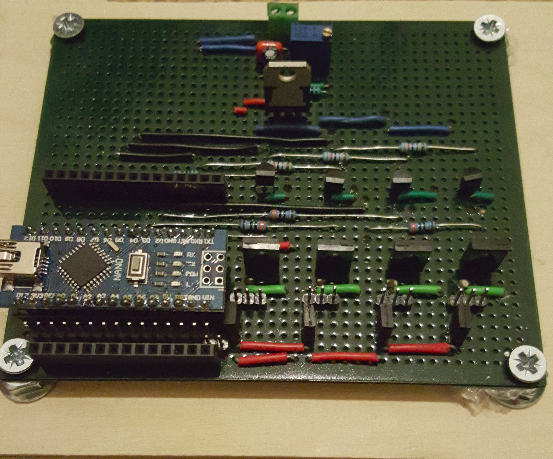
\includegraphics[width=60mm,height=50mm]{{{ImagesSSVEP/driver_circuit}.png}}}
    \caption{To κύκλωμα οδήγησης των LED. Ένα arduino Nano δίνει τα σήματα ελέγχου σε καθένα απο τα 8 τρανζίστορ για τον έλεγχο 4 LED συστοιχιών και 4 ενδεικτικών κόκκινων LED. }
    \label{fig:render}
\end{figure}
 
\subsubsection{Λογισμικό Arduino}
\par Όπως έχει αναφερθεί, ο σκοπός που πρέπει να επιτευχθεί είναι κάθε συστοιχία να αναβοσβήνει με την δικής της συχνότητα ανεξάρτητα από τις άλλες. Είναι σημαντικό να υπάρχει απόλυτη ακρίβεια στην συχνότητα, και ευκολία στην επιλογή της κάθε μίας, για να διευκολυνθεί η διαδικασία των πειραματισμών. Προς την ίδια κατεύθυνση θέλουμε να υπάρχει και η δυνατότητα επιλογής διαφορετικού duty cycle για κάθε συστοιχία καθώς,  όπως θα φανεί και στην συνέχεια, επηρεάζει την ποιότητα των SSVEP σημάτων. Ενώ είναι πολύ εύκολο να επιτευχθεί η δημιουργία τετραγωνικού παλμού σε μια ψηφιακή έξοδο του Arduino, πχ ρυθμίζοντας ακριβώς τον χρόνο που θα είναι On και Off με την χρήση της εντολής delay(), η επέκταση αυτής της λειτουργίας και σε άλλες εξόδους ταυτόχρονα απαιτεί την χρήση την χρήση ενώς thread για κάθε διαφορετική έξοδο, τα οποία να εργάζονται παράλληλα. Για αυτό το λόγο χρησιμοποιήθηκε η βιβλιοθήκη Timer του Simon Monk η οποία επιτελεί αυτόν ακριβώς τον σκοπό. Παρόλαυτά δεν παρέχεται η δυνατότητα επιλογής duty cycle, το οποίο παραμένει σταθερά στο $50\%$. Για τον λόγο αυτό τροποποιήθηκε o πυρήνας της βιβλιοθήκης ετσι ώστε ο χρήστης να μπορεί να θέσει ακριβώς την διάρκεια On και Off του παλμού.  Στην εικόνα \#ΕΙΚΟΝΑ φαίνεται η δημιουργία παλμού με την χρήση της delay(), της βιβλιοθήκης Timer.
\par EIKONA

\par Τέλος, επειδή η κατάσταση  των LED πρέπει να ελέγχεται πλήρως από την διεπαφή, η οποία θα είναι γραμμένη σε  Python, χρησιμοποιήθηκε η βιβλιοθήκη Pyserial, έτσι ώστε η διεπαφή και το Arduino να επικοινωνούν σειριακά μέσω της USB θύρας. Με αυτό τον τρόπο είναι δυνατός ο έλεγχος της εκκίνησης η της παύσης των LEDs, καθώς και των κόκκινων ενδεικτικών LEDs.

\begin{table}
	\centering
    \begin{tabular}{| l | l | l | l |}
    \hline
    \textbf{Metric} & \textbf{Value} \\ \hline
    Accuracy & 77.95\% \\ \hline
    Recall & 0.91 \\ \hline
    Precision & 0.87 \\ \hline
    F1-score & 0.88 \\
    \hline
    \end{tabular}
	\caption{Αποτελέσματα 4 μετρικών για την ανίχνευση αντικειμένων πάνω σε όλα τα βίντεο του συνόλου δεδομένων test που χρησιμοποιήσαμε. Παρατηρούμε ότι με σύζευξη λόγου και εικόνας μπορούμε να πετύχουμε ικανοποιητικά αποτελέσματα, πολύ πιο εύρωστα από ό,τι με χρήση μόνο ενός από τους δύο τρόπους.}
	\label{tab:ObjeResult}
\end{table}

%\cite{lawrence_waves}
\end{document}
